\chapter{Relationen und Abbildungen}
\begin{definition}[Relation]
Seien $A$ und $B$ zwei nichtleere Mengen und $R \subseteq A \times B$. Dann nennt man $R$ eine \emph{Relation} auf $A \times B$. Ist $A = B$ nennt man $R$ eine Relation auf $A$.
\end{definition}

Eine Relation definiert eine Bezihung zwischen den Elementen aus $A$ und  den Elementen aus $B$, die im Paar $\rk{x, y} \in R$ enthalten sind.

Es lässt sich für jedes Paar $\rk{x, y} \in A \times B$ feststellen, ob $\rk{x, y} \in R$ oder $\rk{x, y} \notin R$, also ob die gegebene Beziehung vorhanden ist oder nicht.

Besteht die Beziehung $R$ zwischen $x$ und $y$ schreibt man statt $\rk{x, y} \in R$ auch $xRy$.

\section{Darstellung von Relationen}
$A$ und $B$ seien endliche Mengen und $R$ eine Relation auf $A \times B$. Dann kann die Rleation gegeben sein durch
\begin{enumerate}
\item Beschreibung durch Worte $xRy$ wird zu \enq{$x$ steht in Relation zu $y$}.
\item Eine Menge geordneter Paare $R = \gk{\rk{x_1, y_1}, \rk{x_2, y_2}, \dots}$.
\item Einen gerichteten Graphen. Die Elemente von $A$ und $B$ werden als Punkte/Knoten eingezeichnet. Wenn $\rk{x, y} \in R$ zeichnen wir einen Pfeil von $x$ nach $y$. Ein Pfeil heißt in diesem Fall auch Kante.
\item Eine Matrix. Zuerst müssen die Elemente von $A$ und $B$ durchnummeriert werden $A = \gk{x_1, x_2, \dots, x_n}$, $B = \gk{y_1, y_2, \dots, y_m}$. Dann kann man die Wahrheitswerte $M_{ij}$ definieren
	\[M_{ij} = 
	\begin{cases}
	\tx{wahr} & \tx{falls } \rk{x_i, y_j} \in R\\
	\tx{falsch} & \tx{falls } \rk{x_i, y_j} \notin R
	\end{cases}\]
	\[i \in \gk{1, 2, \dots, n}, j \in \gk{1, 2, \dots, m}\]
	Diese Wahrheitswerte kann man in eine Matrix mit $n$ Zeilen und $m$ Spalten eintragen (siehe Abbildung~\vref{fig:Matrixdarstellung_einer_Relation}).
	\begin{figure}[htb]
	\[\begin{pmatrix}
	M_{11} & M_{12} & \cdots & M_{1m}\\
	M_{21} & M_{22} & \cdots & M_{2m}\\
	\vdots & \cdots & \ddots & \vdots\\
	M_{n1} & \cdots & \cdots & M_{nm}
	\end{pmatrix}\]
	\caption{Matrixdarstellung einer Relation}
	\label{fig:Matrixdarstellung_einer_Relation}
	\end{figure}
\end{enumerate}

\begin{example}
Wir betrachten \emph{ein} Beispiel in allen Darstellungen
\begin{enumerate}
\item $R$ sei definiert durch $x \klgl y$ mit $x \in A = \gk{1, 2, 3}$, $y \in \gk{0, 2, 4, 6}$.
\item $R = \gk{\rk{1,0}, \rk{2,0}, \rk{3,0}, \rk{2,2}, \rk{3,2}}$ (siehe Abbildung~\vref{fig:Darstellung_einer_Relation_als_Menge_geordneter_Paare}).
	\begin{figure}[htb]
	\centering
	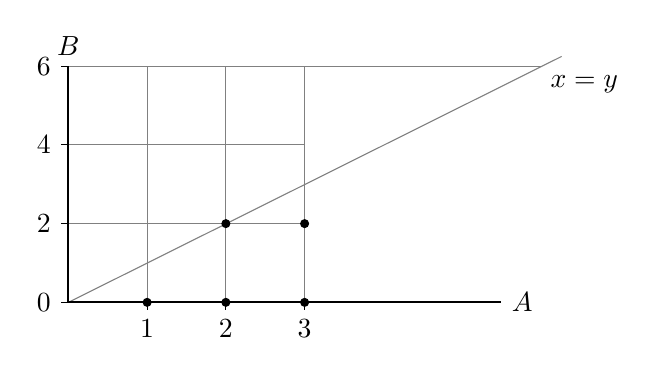
\begin{tikzpicture}
\foreach \x in {1,2,3}
\draw (\x,0.1) -- (\x,-0.1) node[below] {$\x$};

\foreach \x/\t in {0/0,1/2,2/4,3/6}
\draw (0.1,\x) -- (-0.1,\x) node[left] {$\t$};

\draw[color=gray] (0,1) -- (3,1);
\draw[color=gray] (0,2) -- (3,2);
\draw[color=gray] (1,0) -- (1,3);
\draw[color=gray] (2,0) -- (2,3);
\draw[color=gray] (3,0) -- (3,3);
\draw[color=gray] (0,0) -- (26.5:7);
\draw[color=gray] (0,3) -- (6,3) node[below right,color=black] {$x = y$};

\foreach \x/\y in {0/1,0/2,0/3,1/2,1/3}
\draw[fill=black] (\y,\x) circle (0.05);

\draw[thick] (0,3) node[above] {$B$} -- (0,0) -- (5.5,0) node[right] {$A$};
\end{tikzpicture}

	\caption{Darstellung einer Relation als Menge geordneter Paare}
	\label{fig:Darstellung_einer_Relation_als_Menge_geordneter_Paare}
	\end{figure}

\item Siehe Abbildung~\vref{fig:Darstellung_einer_Relation_als_Gerichteter_Graph}.
	\begin{figure}[htb]
	\centering
	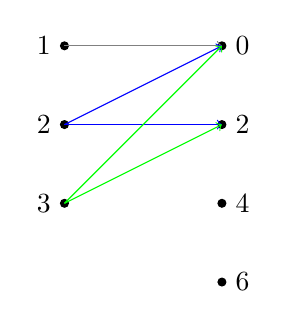
\begin{tikzpicture}
\foreach \y/\t in {0/1,-1/2,-2/3}
{
	\draw[fill=black] (0,\y) circle (0.05);
	\node at (-0.05,\y) [left] {$\t$};
}

\foreach \y/\t in {0/0,-1/2,-2/4,-3/6}
{
	\draw[fill=black] (2,\y) circle (0.05);
	\node at (2.05,\y) [right] {$\t$};
}

\draw[->,color=gray] (0,0) -- (2,0);

\draw[->,color=blue] (0,-1) -- (2,0);
\draw[->,color=blue] (0,-1) -- (2,-1);

\draw[->,color=green] (0,-2) -- (2,0);
\draw[->,color=green] (0,-2) -- (2,-1);
\end{tikzpicture}

	\caption{Darstellung einer Relation als Gerichteter Graph}
	\label{fig:Darstellung_einer_Relation_als_Gerichteter_Graph}
	\end{figure}

\item Siehe Abbildung~\vref{fig:Darstellung_einer_Relation_als_Matrix}.
	\begin{figure}[htb]
	\centering
	\begin{tikzpicture}
\node at (0,0) [right] {
$\begin{pmatrix}
w & f & f & f\\
w & w & f & f\\
w & w & f & f
\end{pmatrix}$};

\node at (-0.2,0) [left] {$A$};
\node at (0.2,0.5) [left] {$1$};
\node at (0.2,0) [left] {$2$};
\node at (0.2,-0.5) [left] {$3$};

\node at (1.5,0.75) [above] {$B$};

\node at (0.65,-0.75) [below] {$0$};
\node at (1.25,-0.75) [below] {$2$};
\node at (1.85,-0.75) [below] {$4$};
\node at (2.45,-0.75) [below] {$6$};
\end{tikzpicture}

	\caption{Darstellung einer Relation als Matrix}
	\label{fig:Darstellung_einer_Relation_als_Matrix}
	\end{figure}
\end{enumerate}
\end{example}

\begin{note}
Falls $A = B = \gk{1, 2, 3}$ mit gleicher Relation wie im Beispiel, kann statt der Darstellung in Abbildung~\vref{fig:Darstellung_einer_Relation_als_Gerichteter_Graph} auch die Diagramm in Abbildung~\vref{fig:Alternative_Darstellung_einer_Relation_als_Gerichteter_Graph} gezeichnet werden.
\begin{figure}[htb]
\centering
\begin{automat}
\node[state] (2) {$2$};
\node[state, right of=2] (3) {$3$};
\node[state, above right of=2] (1) {$1$};

\path[->] (2) edge (1);
\path[->] (2) edge[loop left] ();

\path[->] (3) edge (1);
\path[->] (3) edge (2);
\path[->] (3) edge[loop right] ();

\path[->] (1) edge[loop right] ();
\end{automat}

\caption{Alternative Darstellung einer Relation als Gerichteter Graph}
\label{fig:Alternative_Darstellung_einer_Relation_als_Gerichteter_Graph}
\end{figure}
\end{note}

\begin{exercise}
Es sei $R$ die Relation auf $A \ceq \gk{1, 2, 3, 4}$, die dadurch definiert ist, dass $xRy$ genau dann gilt, wenn $x + 2y$ ungerade ist. Stellen sie $R$ auf jede der folgenden Arten dar:
\begin{itemize}
\item als Menge geordneter Paare
\item als gerichteten Graphen
\item als Matrix
\end{itemize}
Für die Lösung siehe \vref{loe:Aufgabe_1_4}.
\label{exc:Aufgabe_1_4}
\end{exercise}
